\begin{figure}[ht]
    \centering
    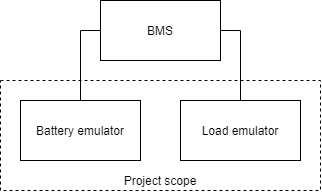
\includegraphics[scale=0.7]{System_context_diagram.png}
    \caption{System context diagram}
    \label{fig:system_context_diagram}
\end{figure}

The goal of this project is to design a programmable hardware system that presents a BMS with a "battery" and a "load" (see figure \ref{fig:system_context_diagram}). The hardware system emulates the battery and load. By using only software changes the hardware system should be able to emulate a battery with a different chemistry, capacity and cell topology. Likewise the hardware system should be able to emulate different loads from electronics through to motors under varying load.

At the end of the project it is expected that a battery and load emulator prototype is delivered. As well as a research report on existing battery and load emulators and the requirements for future battery and load emulators.
% As well as a research report on existing hardware emulators and the requirements for future emulators.

\section{Research questions}
To be able to accomplish these deliverables the following research questions have been derived:
\begin{itemize}
    \item What different battery chemistries are there?
    \item How do different battery chemistries behave?
    \item What different battery cell topologies are there?
    \item How do different battery cell topologies behave?
    \item How do different battery capacities behave?
    \item What kind of loads are there?
    \item How do different loads behave?
    \item How to control the voltage, current and phase to emulate a battery cell via software changes?
    \item How to control the voltage, current and phase to emulate a load via software changes?
    \item What battery emulators already exist?
    \item What load emulators already exist?
    \item What are the requirements for future emulators?
\end{itemize}

\section{Requirements}
For this project the following requirements have been specified, following the MoSCoW method. 

\begin{longtable}{|c|p{10cm}|c|c|}
    \hline
    \textbf{ID} & \textbf{Requirement} & \textbf{Priority} & \textbf{Status}\\ \hline 
    \textbf{U1} & The hardware is able to emulate a battery with a specific lithium-ion chemistry and capacity & Must & Proposed\\ \hline
    \textbf{U2} & The hardware is flexible enough to require only software changes to emulate a battery with a different chemistry, a different capacity, and a different cell topology & Must & Proposed\\ \hline
    % \textbf{U3} & The hardware is able to emulate different loads: from electronics through to motors under varying load & Must & Proposed\\ \hline
    \textbf{U3} & The hardware system is able to adjust the load impedance characteristic curve & Must & Proposed\\ \hline
    \textbf{U4} & The hardware system is tested & Must & Proposed\\ \hline
    \textbf{U5} & The hardware is able to control the voltage, current and phase independently & Must & Proposed\\ \hline
    \textbf{U6} & The hardware contains a BMS & Won't & Proposed\\ \hline
\end{longtable}

